\documentclass[12pt]{article}


\usepackage{fullpage,enumitem,amsmath,amsfonts,amssymb,amsthm,graphicx}
\usepackage{array} % Improves `tabular` and `array` environments
\usepackage{pict2e} % Allows \linethickness{...} in diagonal lines
\usepackage{diagbox}
\usepackage{breqn} % Fit equations in pages
\usepackage[linewidth=1pt]{mdframed}

\newcommand{\Z}{\mathbb{Z}}
\newcommand{\R}{\mathbb{R}}
\newcommand{\C}{\mathbb{C}}
\newcommand{\Q}{\mathbb{Q}}
\newcommand{\N}{\mathbb{N}}
\newcommand{\F}{\mathbb{F}}
\newcommand{\E}{\mathbb{E}}
\newcommand{\Exp}[1]{\text{exp}(#1)}
\newcommand{\Diag}[1]{\text{Diag}(#1)}
\newcommand{\norm}[1]{\left\Vert #1\right\Vert}
\newcommand{\Span}[1]{\text{Span}(#1)}
\newcommand{\Cov}[1]{\text{Cov}(#1)}

\newenvironment{solution}{\vspace{0.2cm} \textbf{Solution.}}{}
\setlength{\parindent}{0pt}

% ------------------------------------------------------------------- %

\title{\vspace{-3cm}2801.001 Spring 2018 Homework 2 }
\author{Martin Arienmughare -- \texttt{moa258}\\
		Madhur Bhattad-- \texttt{mb6854}\\
		Louis Guigo -- \texttt{lg2894}\\
		Mario Zhu -- \texttt{mz833}}
\date{May 2018}

% ------------------------------------------------------------------- %

\begin{document}

\maketitle

\textbf{Submission instructions:} Same groups as HW1. Refer to instructions from TA.
\\

\textbf{Note:} Problems 1 and 2 require the datafile posted online which contains prices and implied volatilities of one-year (349 calendar days) listed options on the Nasdaq 100 index (NDX), as well as other market data.

\noindent
\rule{\linewidth}{0.4pt}

\section*{Problem 1}

	\begin{enumerate}[label=(\alph*)]

		\item Estimate the market price of the $5\%$ call spread (i.e.\ with strikes ATM and $5\%$ OTM). What about the $5\%$ put spread?

		\begin{solution}

		The Nasdaq 100 data provided allows us to get the buy and sell prices of ATM (strike 5050) and $5\%$ OTM (strikes 5200 and 5750) call and put prices.
		
		\begin{enumerate}
			\item[$\bullet$] Selling ATM Call: $337.1$.
			
			\item[$\bullet$] Selling ATM Put: $326.1$.
			
			\item[$\bullet$] Buying 5\% OTM Call: $478.1$.
			
			\item[$\bullet$] Buying 5\% OTM Put: $428.3$.
		\end{enumerate}
	
		Therefore, the buy prices of the 5\% call and put spreads are:
		
		\begin{enumerate}
			\item[$\bullet$] 5\% call spread: $478.1 - 337.1 = 141.0$.
			
			\item[$\bullet$] 5\% put spread: $428.3 - 326.1 = 100.2$.
		\end{enumerate}		

		\end{solution}
	
	\newpage

		\item If you were to price the spreads in the Black-Scholes model using a single volatility parameter $\sigma$, what value of $\sigma$ would match the theoretical price with the market price? Comment on your results.
	
		\begin{solution}

		Applying a Black-Scholes pricing formula would lead to the following theoretical prices for the 5\% call spread (5\% put spread resp.):
		
		\begin{dmath*}
		CS(K,0.95K) = C(0.95K) - C(K) =  S_t N(d_1(0.95K)) - 0.95K e^{-r(T-t)}N(d_2(0.95K)) - (S_t N(d_1(K)) - K e^{-r(T-t)}N(d_2(K)))
		\end{dmath*}
	
		\begin{dmath*}
		PS(K,1.05K) = P(1.05K) - P(K) = 1.05K e^{-r(T-t)} N(-d_2(1.05K)) - S_t N(-d_1(1.05K)) - (K e^{-r(T-t)} N(-d_2(K)) - S_t N(-d_1(K)))
		\end{dmath*}
		where
		\begin{align*}
		d_1(K) &= \frac{1}{\sigma\sqrt{T - t}}\left[\ln\left(\frac{S_t}{K}\right) + \left(r + \frac{\sigma^2}{2}\right)(T - t)\right] \\
		d_2(K) &= d_1 - \sigma\sqrt{T - t}
		\end{align*}
		$\sigma$ is the implied volatility that one can choose to equate theoretical prices to market prices.

		Using a solver, we get $\sigma_{CS} = 14.13\%$ using the 5\% call spread and $\sigma_{PS} = 17.10 \%$ using the 5\% put spread.
		
		These levels are relatively close to the implied volatility quoted for ATM (15.4 \%) and 5\% OTM options (14\% to 16.7\%)

		\end{solution}

	\end{enumerate}

\newpage

\section*{Problem 2}

	\begin{enumerate}[label=(\alph*)]

		\item Using the numerical package of your choice, calibrate the parameters of the SVI model against the market-implied volatility data. Show a comparative graph of the SVI curve and the actual implied volatility data points.

		\begin{solution}
		
		The SVI model reads: 
		$$ \sigma^* = \sqrt{a + b \left( \rho (x - m)  + \sqrt{(x-m)^2 + s^2} \right)} $$

		To calibrate its parameters ($a, b, \rho, m, s$) we perform the following least square optimization against market data (both puts and calls), with the following constraints to avoid arbitrage:
        \begin{subequations}
        	\begin{alignat*}{2}
        	&\!\min_{a,b,\rho,m,s}        &\quad& \sum_{i=1}^{n} \left[ \sigma_{\text{SVI}}^{\star^2}(k_i,T;a,b,\rho,m,s) - \sigma_{\text{Market}}^{\star^2}(k_i,T)\right]^2\\
        	&\text{subject to} &      & a,b \geq 0,\\
        	&                  &      & -1 \leq \rho \leq 1,\\
        	&                  &      & s > 0,\\
        	&                  &      & b(1 + |\rho|)T \leq 4.
        	\end{alignat*}
        \end{subequations}
    	
		Using a Sequential Least Squares Programming method in \texttt{scipy.minimize}, we obtain: $$a = 0.000364, b = 2.55, \rho = 0.961, m = 0.239, s = 0.0149$$
		
		The quality of the fit is very good:
		
		\begin{center}
			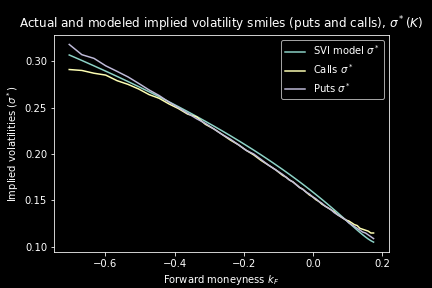
\includegraphics[width=0.5\textwidth]{SVI_calibrated}
		\end{center}

		\end{solution}

		\item Compute or estimate the price of an at-the-money digital call option paying off $\$1$ if in one year NDX is greater than its current spot level, and zero otherwise: (i) in the Black-Scholes model, (ii) using $\pm 1\%$ call spreads, (iii) using the smile-adjusted formula on page 19.

		\begin{solution}

		\begin{enumerate}
			\item[$\bullet$] Black-Scholes model: $D_{BS}(S_t,K,r,T,\sigma)=e^{-rT}N(d_2)$. We obtain: 0.495.
			\item[$\bullet$] Using $\pm 1\%$ call spreads. We obtain: 0.419.
			\item[$\bullet$] Using smile-adjusted formula: $D(S_t,K,r,T) = (D_{BS}- V_{BS} \times \frac{\partial \sigma^*}{\partial K})(S_t,K,r,T,\sigma^*(K,T))$, where $V_{BS}$ is the Black-Scholes vega, $V_{BS} = S_t \frac{e^{-\frac{d_1^2}{2}}}{\sqrt{2\pi}} \sqrt{T-t}$. We obtain: 0.590.
		\end{enumerate}

		\end{solution}

		\item Graph the implied distribution corresponding to the SVI model calibration.

		\begin{solution}

			As expected, the density obtained from options prices is right skewed and has fatter tails than the Black-Scholes lognormal random variable:
			
			\begin{center}
				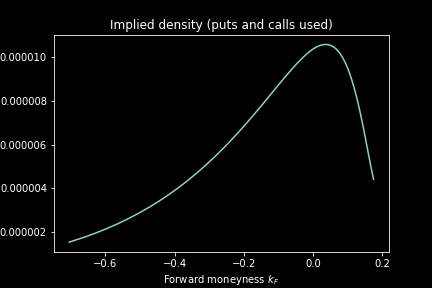
\includegraphics[width=0.5\textwidth]{implied_distribution}
			\end{center}

		\end{solution}

		\item Use the implied distribution to compute the price of the following European exotic options, where $X_0$ is the current index level and $X_T$ is the final index level:

		\begin{solution}
			
			Knowing the implied distribution of an underlying, the value of a derivative $f_t$ at time $t$ with a certain payoff $f(S_T)$ at maturity $T$ is given by discounted the expected payoff under this measure: $f_t = e^{-r(T-t)}\mathbb{E}(f(S_T))$. We apply this to the following cases:

			\begin{enumerate}[label=(\roman*)]

				\item Digital call defined in question (b);

				Its payoff is just $\mathbb{I}(X_T > K)$. We obtain: $0.0131$.

				\item "Reverse convertible" paying off $\max\left(100\%, 100\% + p \times \frac{X_T- X_0}{X_0}\right)$ if $\frac{X_T}{X_0} > 75 \%$ and $\frac{X_T}{X_0}$ otherwise, where $p = 50\%$. Then solve for $p$ to get a price of $100\%$;

				With $p=0.5$, we obtain: $0.0230$.
				
				To get a price of $1.0$, we just apply a rootfinding technique to the payoff to which we substract $1.0$, we get: $p=0.5$.
				
				
				\item Option paying off $\max\left(0, \frac{X_T- X_0}{X_T}\right)$;

				We get: $0.000796$.

				\item Log-contract paying off $-2\log\left(\frac{X_T}{X_0}\right)$. Price interpretation;

				We get: $0.00429$.
				
				Assuming arbitrage (it is the case since we fitted the SVI model), this can be interpreted as the current expected total return gained on the stock over the life-time of the option, i.e.\ 0.429 \% over 1 year.
			\end{enumerate}

		\end{solution}

	\end{enumerate}

\newpage

\section*{Problem 3}
Find conditions on the SVI model parameters to satisfy Lee’s asymptotic bounds on p$.\ 22$: 
$$\sigma^{\star^2} (k_F,T) \leq \frac{\beta}{T} |\log{k_F}|,\, \beta \in [0,2]$$

	\begin{solution}

	In the SVI model, the implied variance reads:
	$$ \sigma^{*^2}(a,b,\rho,m,s; x) = a + b(\rho(x-m) + \sqrt{(x-m)^2 + s^2})$$
	
	The no arbitrage constraints are: 
	$$ a,b \geq 0$$
	$$ |\rho| \leq 1 $$
	$$ s > 0 $$
	$$ b(1 + |\rho|)T \leq 4$$
	
	In order for the variance to be greater than zero, we must ensure that the minimum value of the above expression to be greater than zero.
	
	Since its second derivative is positive, a minimum is obtained by equating its derivative with respect to x as zero. Doing that, we get a minimum value of $$a + b\sigma\sqrt{1-\rho^2}$$
	
	Therefore we get the additional constraint: $$a + b\sigma\sqrt{1-\rho^2} \geq 0$$
	
	Using Lee's asymptotic inequality, as $x$ tends to infinity,
	$$ \sigma^{*^2} \geq \frac{\beta|x|}{T}$$
	
	where $\beta \in [0,2]$.
	
	Taking $x$ to infinity in the expression $\sigma^{*^2} = |x-m|\left(\frac{a}{|x-m|} + b\rho \left(\text{sign}(x-m) + \sqrt{1 + \frac{\sigma^2}{(x-m)^2}} \right)\right)$
	gives that $b(1+\rho) \leq \frac{\beta}{T}$ and $b(1-\rho) \leq \frac{\beta}{T}$.
	
	Therefore we have, $$0 \leq bT(1+\rho) \leq \beta$$ $$0 \leq bT(1-\rho) \leq \beta$$ where $\beta \in [0,2]$.

	\end{solution}

\newpage

\section*{Problem 4}
(Problem $4.3$ p$.\ 56$ in textbook, with corrections): Consider an underlying stock $S$ currently trading at $S_0 = 100$ which does not pay any dividend. Assume the local volatility function is $\sigma_{loc} (t, S) = \frac{0.1 - 0.15 \times \log\left(\frac{S}{S_0}\right)}{\sqrt{t}}$, and that interest rates are zero.

	\begin{enumerate}[label=(\alph*)]
		
		\item Produce the graph of the local volatility surface for spots $0$ to $200$ and maturities $0$ to $5$ years.
		
		\begin{solution}
			
			\begin{center}
				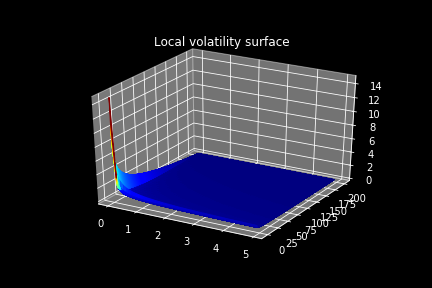
\includegraphics[width=0.5\textwidth]{local_vol}
			\end{center}
			
		\end{solution}
		
		\item Write a Monte-Carlo algorithm to price the following $1$-year payoffs using $252$ time steps and e.g.\ $10,000$ paths:
		
		\begin{solution}
			
			The continuous time formulation of the local volatility model is that the spot price process is a diffusion of the form:
			$$ dS_t = \mu_t dt + \sigma_{loc} (t,S_t) dW_t$$
			
			In our case, we have the expression of the local volatility and there is no interest rate and no dividend yield. Therefore, $\mu_t = 0$ and:
			$$ dS_t =  \frac{0.1 - 0.15 \times \log\left(\frac{S}{S_0}\right)}{\sqrt{t}} dW_t$$
			
			We use a Euler scheme to simulate this SDE, and then apply a Monte Carlo technique to price the following derivatives:
			
			\begin{enumerate}[label=(\roman*)]
	
				\item "Capped quadratic" option: $\min\left(1,\frac{S_1^2}{S_0^2}\right)$;
								
				We get: $0.998$.
				
				\item Asian at-the-money-call: $\max\left(0, \frac{S_{0.25} + S_{0.5} + S_{0.75} + S_1}{4 \times S_0} - 1\right)$;
				
				We get: $0.000914$.
				
				\item Barrier call: $\max(0, S_1 - S_0)$ if $S$ always traded above $80$ using $252$ daily observations, 0 otherwise;
				
				We get: $0.0979$.
				
			\end{enumerate}
			
		\end{solution}
		
	\end{enumerate}

\newpage

\section*{Problem 5}
The payoff of a $1$-year at-the-money call on the geometric average return of two non-dividend paying stocks $X, Y$ is given as:

$$ f(X_T,Y_T) = \max\left(0, \sqrt{\frac{X_T Y_T}{X_0 Y_0}} - 1\right) = \frac{1}{\sqrt{X_0 Y_0}}\max\left(0, \sqrt{X_T Y_T} - \sqrt{X_0 Y_0}\right)$$

where $T = 1$ year and $X_t, Y_t$ are the respective underlying spot prices of $X, Y$ at any time $t$.
	
	\begin{enumerate}[label=(\alph*)]
		
		\item Derive analytical formulas for the call value at any time $0 \leq t \leq T$ in the Black-Scholes model with constant correlation $\rho$ (cf.\ Section $6-4$ in the textbook, to be covered during Session $5$.)
		
		\begin{solution}
			
			In a Black-Scholes world, these two correlated stocks have the dynamics:
			$$ dX_t = (r-\mu_1) X_t dt + \sigma_1 X_t dW_t$$
			$$ dY_t = (r-\mu_2) Y_t dt + \sigma_2 Y_t (\rho dW_t + \sqrt{1 - \rho^2}dZ_t)$$
			
			where r is the risk-free rate, $\mu_1, \mu_2$ are the dividend yields (equal to 0 here by assumption), $\rho$ is the constant correlation between $X$ and $Y$, and $W,Z$ are two uncorrelated Brownian motions.
			
			The value of this call is given by: $f_t = \frac{e^{-r(T-t)}}{\sqrt{X_0 Y_0}} \mathbb{E}\left(\max\left(0, \sqrt{X_T Y_T} - \sqrt{X_0 Y_0}\right) \vert X_t,Y_t \right)$
			
			The geometric average of two lognormal is still lognormal. Indeed, for $\alpha > 0$, let us apply Itô-Doeblin formula to the process $V_t = (X_tY_t)^{\alpha}$:
			
			We obtain:
			
			\begin{dmath*}
			dV_t = \left(r - \left(\mu_{X,Y} + \left(1-\alpha\right) \left(r - \mu_{X,Y} + \frac{1}{2} \sigma_{X,Y}^2 \right)\right)\right) V_t dt + \alpha V_t \left( \sigma_1 dW_t + \sigma_2 \left(\rho dW_t + \sqrt{1 - \rho^2}dZ_t \right)\right)
			\end{dmath*}
		
			where $\mu_{X,Y} = \mu_1 + \mu_2 -r -\rho \sigma_1 \sigma_2$ and $\sigma_{X,Y} = \sqrt{\sigma_1^2 + \sigma_2^2 + 2\rho \sigma_1 \sigma_2}$.
			
			
			In our case, we assume no dividend ($\mu_1 = \mu_2 = 0$) and $\alpha =\frac{1}{2}$, so the dynamics of $V_t$ simplifies to:
			\begin{dmath*}
			dV_t = \left(r - \frac{1}{4} \left(\sigma_1^2 + \sigma_2^2\right)\right) V_t dt + \frac{1}{2} V_t \left( \sigma_1 dW_t + \sigma_2 \left(\rho dW_t + \sqrt{1 - \rho^2}dZ_t \right)\right)
			\end{dmath*}
			
			If we call $dB_t = \frac{\sigma_1 dW_t + \sigma_2 \left(\rho dW_t + \sqrt{1 - \rho^2}dZ_t \right)}{\sigma_{X,Y}}$, where again $\sigma_{X,Y} = \sqrt{\sigma_1^2 + \sigma_2^2 + 2\rho \sigma_1 \sigma_2}$, $B_t$ is a Brownian and we have:
			\begin{dmath*}
			dV_t = \left(r - \frac{1}{4} \left(\sigma_1^2 + \sigma_2^2\right)\right) V_t dt + \frac{1}{2} \sigma_{X,Y} V_t dB_t
			\end{dmath*}

			Under this form, we see that $V_t = \sqrt{X_t Y_t}$ follows a lognormal distribution.
			
			Therefore, the price of the option is given by the following Black-Scholes formula:
			$$ f_t = \frac{1}{\sqrt{X_0 Y_0}} \left(e^{-\frac{1}{4} \left(\sigma_1^2 + \sigma_2^2\right)(T-t)}\sqrt{X_t Y_t} N(d_1^*) + \sqrt{X_0 Y_0} e^{-r(T-t)}N(d_2^*)\right)$$
			where
			\begin{dmath*}
			d_1^*(K) = \frac{2}{\sqrt{\sigma_1^2 + \sigma_2^2 + 2\rho \sigma_1 \sigma_2}\sqrt{T - t}}\left[\ln\left(\frac{\sqrt{X_t Y_t}}{\sqrt{X_0 Y_0}}\right) + \left(r - \frac{1}{4} \left(\sigma_1^2 + \sigma_2^2\right) + \frac{\sigma_1^2 + \sigma_2^2 + 2\rho \sigma_1 \sigma_2}{8}\right)(T - t)\right]
			\end{dmath*}
			\begin{dmath*}
			d_2^*(K) = d_1^* - \frac{1}{2} \sqrt{\sigma_1^2 + \sigma_2^2 + 2\rho \sigma_1 \sigma_2} \sqrt{T - t}
			\end{dmath*}
			
		\end{solution}
		
		\item Compute the value of the call using a $5\%$ interest rate, $20\%$ volatility for $X$, $30\%$ volatility for $Y$, and $\rho = 0.4$. Use finite differences to estimate the deltas, gammas and cross-gamma of the call.
		
		\begin{solution}
			
			Using unit values for $X_0,Y_0,X_t,Y_t$, and $\sigma_1 = 20\%$, $\sigma_2 = 30 \%$ and $\rho = 0.4$, we get: $1.06$.
			
			For the same values, finite differences (although explicit greeks could be computed) give: $\delta_X = 2.156, \delta_Y = 2.156, \gamma_X = -1.428, \gamma_Y = -1.428, \gamma_{XY} = 1.428$.
			
		\end{solution}
		
		\item You purchased the call on a $\$10,000,000$ notional. What actions would you take to delta-hedge your position? What would then be your instant $P\&L$ in the following matrix of scenarios. Generally, graph your instant $P\&L$ against percent changes $x, y$ in underlying stock prices.
		
		\begin{solution}
			
			The first-order underlying risks are represented by the delta vector. It can be cancelled by buying/selling shares of each underlying by an amount equal to the corresponding delta.
			
			One must realize that these positions DO NOT hedge the first-order correlation risk that is rather cumbersome to deal with. We would have to cancel our correlation vega, but it changes as cross-gammas (and eventually cross-volgas) are neutralized.
			
			Below are the table and the plot of our instant $P\&L$ against percent changes $x, y$ in underlying stock prices (we used the values of question b) for the volatilities, the correlation, the maturity and the risk-free rate).
			
			Note that we assumed that everything happened on a short timeframe, hence we neglected interest rate effects (the true $P\&L$ would be $d\Pi - r\Pi dt$, where $\Pi$ is the money borrowed to set up initially our delta-hedged portfolio).
			
			With these parameters:
			
			\begin{enumerate}
				\item[$\bullet$] Price of the call at time 0: $5937170.$
				\item[$\bullet$] Initial deltas (X,Y): $1.2564, 1.2564$
				\item[$\bullet$] Delta-hedged portolio setup cost $\Pi$: $19192049.204$
			\end{enumerate}
		\[
		\linethickness{1pt}
		\setlength{\arrayrulewidth}{1pt}
		\begin{tabular}{|c|c|c|c|}
			\hline
			\backslashbox{$\quad X$}{$\quad Y$} & $\qquad -5\% \qquad$ & \qquad $+1\%\qquad$ & \qquad $+5\%\qquad$ \\ \hline
			$-5\%$ & 1268867 & 509080 & 14286 \\ \hline
			$+1\%$ & 509080 & -250705 & -745500 \\ \hline
			$+5\%$ & 14286 & -745500 & -1240294 \\ \hline
		\end{tabular}
		\]
		
		Rebalancing this delta-hedged portfolio costs money when the stocks go up, and brings money when they go down. This is consistent since we are long the call.
		
		\begin{center}
			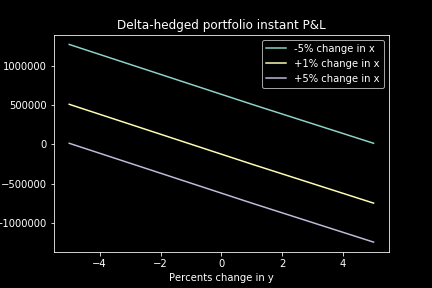
\includegraphics[width=0.5\textwidth]{instant_pnl}
		\end{center}
		
		\end{solution}
	
	\end{enumerate}

\end{document}